%begin-include

% What I want to talk about in this section?
% - Cells signaling pathways are part of the cell communication system,
% and it allows the cell to perceive the conditions of the environment 
% and also to change its behaviour according to the input signal.
% - The signals perceived by a cell can come from cells that very close
% (including itself), as in synapses or it can travel long distances in 
% the organism, as in hormones.
% - When a signal reaches a cell, it can either activate a receptor in
% the cell membrane or diffuse into the cell.
% - Once this happen, the signal or the activated receptor can trigger
% a sequence of chemical interaction, altering the conformation and 
% state of proteins and also changing the concentration of chemical 
% species in the cell. Ultimately, this chain of effects can alter the 
% behaviour of the cell, what is called signal transduction.
% - Studying signaling pathways is important because they help us 
% understand the mechanisms of a cell, which can for example, elucidate 
% treatments for diseases.
\section{Cell Signaling Pathways}
Cell signaling pathways are part of the complex cell communication 
system, and it allows the cell to perceive the conditions of the 
environment in which it is placed and change its behaviour accordingly.
Signaling pathways participate in the regulation of many cell functions,
including development, division and cell death. Bad functioning 
signaling pathways can also be related to diseases, as in many cases of
cancer.

The signal perceived by a cell can come from cells that are close 
(including the same cell that produced the signal), as in synapses, or 
it can travel long distances in the organism, as in hormones. When a 
signal reaches a cell, it can either penetrate the cell or bind to some 
specific receptor in the membrane. Once either of those events happen, 
the signal or the receptor can trigger a sequence of chemical 
interactions that can include change of conformation of proteins, 
activation or inactivation of proteins, and change of concentration of
chemical species in the cell. Ultimately, this chain of chemical 
reactions caused by the signal can alter the behaviour of the cell, what 
is called signal transduction.

Since signaling pathways participate in many of the cell functions, and 
are also related to diseases, it is important to study those structures
in order to get a better understanding of the cell mechanisms and 
diseases. One approach on the study of the cell signaling pathways is to 
measure the concentration change of proteins that participate on the 
pathway of interest.

% - Western blot is a technique that can indicate the amount of a 
% specific protein that is in a mixture of proteins
% - This technique shows the presence of a protein in a mixture by 
% ``blotting'' these molecules into a membrane. 
% - Repeating the procedure in different times define time-course 
% observations of the protein in a biological experiment.
% - With these observations in hand, the researcher is able to construct 
% a measurement that is relevant to describe the biological experiment. 
% For instance, in a signaling network where a protein is closely 
% related to the behaviour of interest of the cell, this protein is a 
% good candidate as a measure of the system.
\section{Measurements of Proteins in Cell Signaling Pathways}
Western blot is a laboratory technique that can indicate the amount of a
specific protein that is present in a mixture. This technique show the 
presence of a protein in a mixture by ``blotting'' a membrane where the 
molecules of interest are located. We can superficially summarize the 
procedure in the following steps: first a mixture containing a sample of 
cells of interest must be created; second, proteins from the mixture 
should be fixed on the blotting membrane; third, an antibody should bind 
to the target protein molecules; and finally, a method for highlighting 
the bound antibody should be applied. An image of the resulting membrane 
can then be analyzed with computer programs to quantify the relative 
concentration of the protein of interest.

By repeating this procedure in different times it is possible to create 
time-course observations of proteins throughout the biological 
experiment. With this tool, a researcher can choose a set of relevant 
proteins from a signaling network and gain knowledge about the dynamics 
of such chemical species during the experiment. For instance, in a 
signaling network experiment in which it is desired to understand how
the change of concentrations of a species at the beginning of the 
pathway changes the concentration of some species at the end of the 
cascade, then measurements of both are relevant to understand the 
biological experiment. Figure~\ref{fig:western_blot_example} show an 
example of time-course Western blot for an experiment where it is 
desirable to understand how ERK is activated (phosphorylated) as a 
function of levels of Ras-GTP. {\color{blue} TODO: what is ERK, what is
Ras-GTP?}

\begin{figure}[!ht]
\centering
    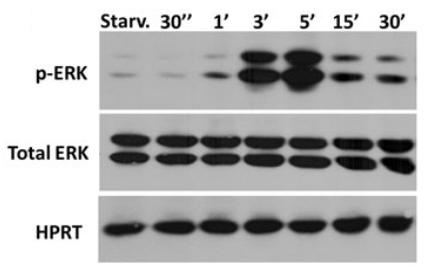
\includegraphics[width=\textwidth]{fundamental_concepts/western_blot.png}
    \caption{Figure {\bf a} shows time-course measurements of ERK and 
    phosphorylated ERK. {\color{blue}HPRT is a TODO: what is it? Finish this caption!} }
    \label{fig:western_blot_example}
\end{figure}

These measurements alone do not always provide means for researchers to 
understand a cell signaling pathway experiment. However, if we create a 
computational models for this signaling networks that is able to 
reproduce experimental data, then it is possible to use this model as a 
summary of the signaling network, which can provide to researchers 
evidences of the biological phenomena.


\section{Dynamic Modeling of Cell Signaling Pathways}
\section{Identification of Cell Signaling Pathways}
\section{State of the Art in Model Selection}
%\section{Bayesian Inference}
%\subsection{Girolami (bioinformatics)}
%\subsection{Kolch}
%\subsection{ABC-Sysbio}
